\documentclass[12pt]{report}
\usepackage[a4paper, margin=0.5in]{geometry}
% \usepackage[a4paper, top=1in, bottom=1in, left=1in, right=1in]{geometry}
\usepackage{graphicx}
\usepackage{amsmath}
\usepackage{titlesec}
\usepackage{caption}
\usepackage{float}
\usepackage{hyperref}
\usepackage{algorithm}
\usepackage{algorithmic}
\setcounter{secnumdepth}{2}
\titleformat{\section}{\normalfont\Large\bfseries}{\thesection.}{1em}{}
\titleformat{\subsection}{\normalfont\large\bfseries}{\thesubsection.}{1em}{}

\title{\textbf{GPS Spoofing and Anti-Spoofing Techniques}}
\author{Aditya Kumar (210070003) \and Joel Anto Paul (210070037) \\
\and \\
{\large Guide: Prof. Sibiraj Pillai}}
\date{}
\usepackage{enumitem}
\setlist{nosep}
\begin{document}

\maketitle

\begin{abstract}
This report investigates advanced GPS spoofing methodologies that go beyond traditional techniques by focusing on signal cancellation and synthetic signal injection. We present a series of experiments based on GNSS-SDR and GPS-SDR tools, exploring the challenges in detection, correlation, fine Doppler estimation, and signal cancellation to demonstrate the viability of spoofing a GPS receiver without increased signal power.
The code has been made available on Github at \url{https://github.com/SnarkyGoblin123/BTP.git}.
\end{abstract}

\section{Introduction}
GPS spoofing involves manipulating GPS signals to mislead a GPS receiver's position fix. While traditionally viewed as a vulnerability, this area also has significant defense applications. Understanding spoofing helps us devise anti-spoofing strategies and strengthen navigation systems against such attacks.
\begin{figure}[H]
    \centering
    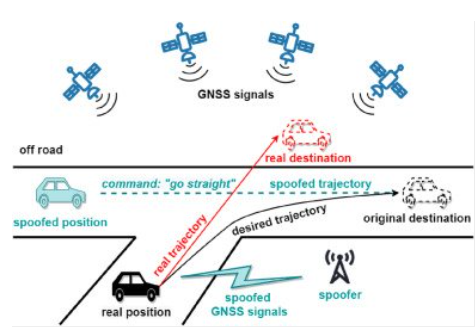
\includegraphics[width=0.6\textwidth]{spoof.png}
    \caption{Illustration of GPS spoofing methodology.}
    \label{fig:spoofing}
\end{figure}

\section{Problem Setting}
A GPS receiver obtains signals from multiple satellites, each transmitting synchronized signals. 
Let $Y$ be the composite received signal and $x_i$ the contribution from satellite $i$. 
The received signal can be modeled as:
\begin{equation}
Y = \sum_{i=1}^{N} \alpha_i x_i e^{j2\pi f_i t} + \nu(t)
\end{equation}
Where:
\begin{itemize}
  \item $N$ is the number of satellites.
  \item $\alpha_i$ is the unknown amplitude of the signal from satellite $i$.
  \item $f_i$ is the Doppler frequency shift for satellite $i$.
  \item $t$ is time.
  \item $\nu(t)$ is the background noise affecting the received signal.
\end{itemize}
The goal is to estimate the $\alpha_i$ values for each satellite, allowing us to manipulate the received signal.
Before diving into the details, we will first discuss the GNSS-SDR framework and the GPS signal structure.
\section{GNSS-SDR Framework}
GNSS-SDR \ref{ref:gnss_sdr}  is an open-source, modular software-defined receiver for Global Navigation Satellite Systems (GNSS). 
It allows real-time processing of raw signal samples captured from radio front ends and outputs positioning and navigation data.
\subsection{Architecture}
\begin{itemize}
  \item \textbf{Modular Design:} Composed of blocks that can be configured and connected in various ways.
  \item \textbf{Signal Processing Blocks:} Each block performs a specific function, such as signal acquisition, tracking, and decoding.
  \item \textbf{Data Flow:} Data flows through the blocks, with each block processing the signal and passing it to the next.
  \item \textbf{Configuration:} Users can configure the receiver to work with different GNSS constellations and signal types.
  \item \textbf{Real-time Processing:} Capable of processing live signals in real-time, making it suitable for various applications.
  \item \textbf{Open-source:} The source code is available for modification and experimentation, allowing researchers to develop new algorithms and techniques.
\end{itemize}

\begin{figure}[H]
    \centering
    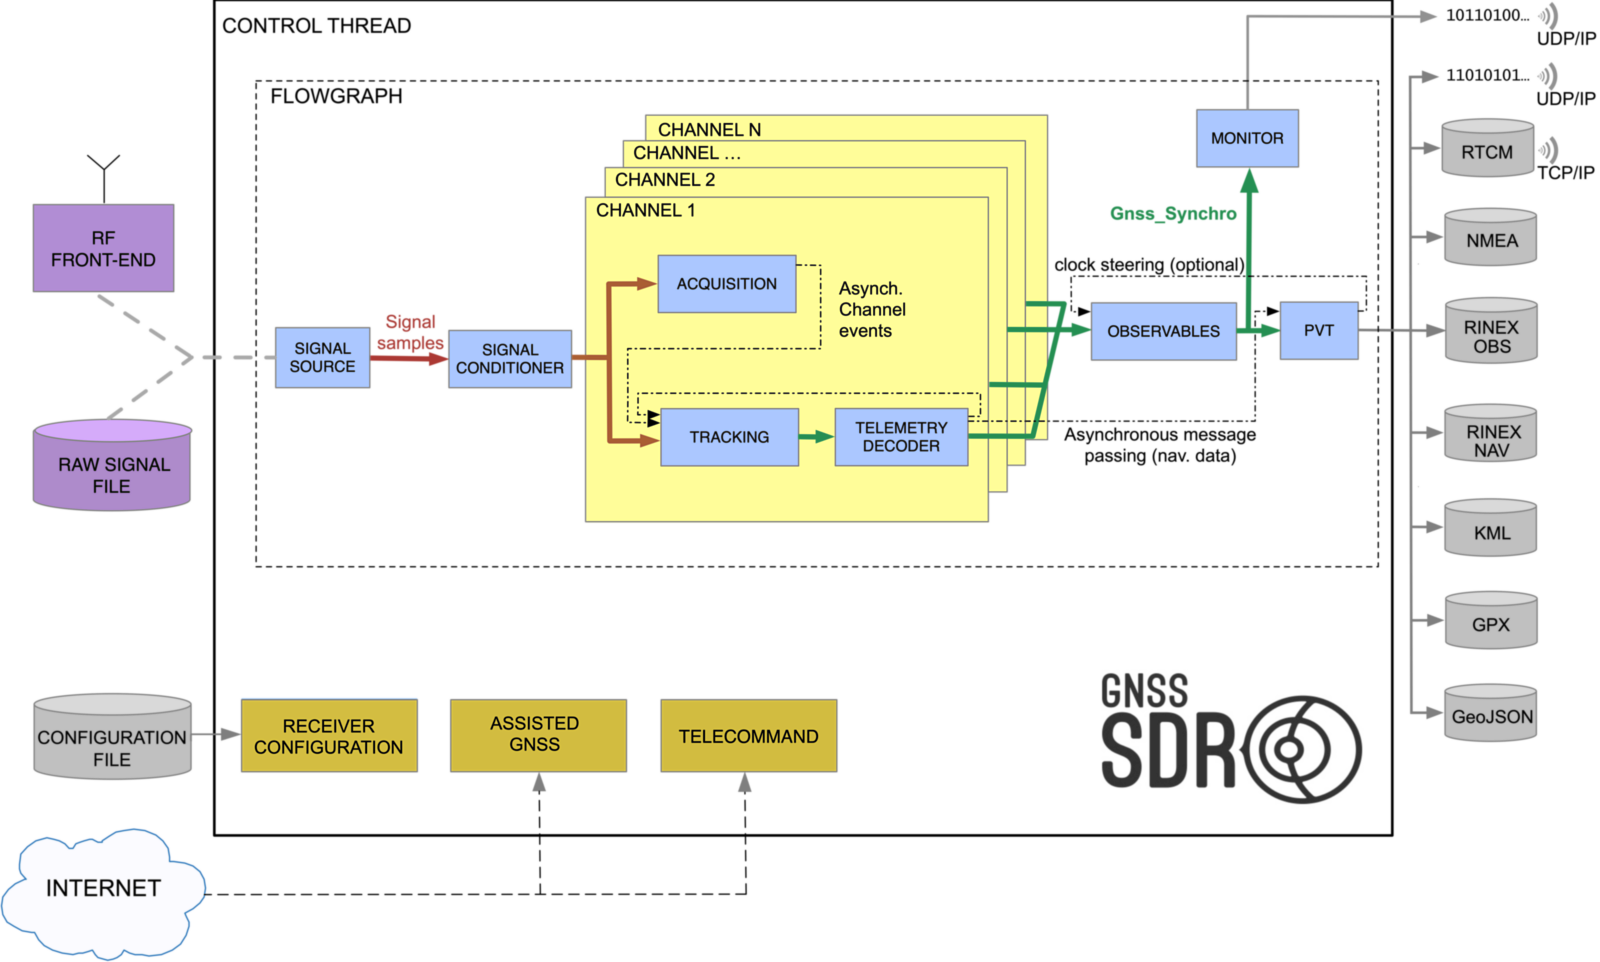
\includegraphics[width=0.6\textwidth]{GNSS_SDR.png}
    \caption{GNSS-SDR Framework Overview.}
    \label{fig:gnss_sdr}
\end{figure}
\subsection{Core Components}
\begin{itemize}
  \item \textbf{Signal Source:} Interfaces with RF front ends or file-based input.
  \item \textbf{Acquisition Block:} Identifies visible satellites and estimates initial Doppler and code phase.
  \item \textbf{Tracking Block:} Maintains lock on satellite signals and refines Doppler/code phase.
  \item \textbf{Decoding Block:} Extracts NAV data including ephemeris and almanac.
  \item \textbf{PVT Computation:} Computes Position, Velocity, and Time (PVT) using decoded satellite data.
\end{itemize}


\subsection{Advantages}
\begin{itemize}
  \item High modularity for rapid experimentation.
  \item Supports both GPS and Galileo constellations.
  \item Allows testing with both live and synthetic datasets.
\end{itemize}

In addition to the above features, GNSS-SDR also provides logging capabilities which helps us identify what went wrong, which satellite signals are present and finally the RINEX observation files
provide useful data such as the doppler shifts. It also outputs the telemetry bits which can be used in exoperiments to verify the presence of the satellites.

\section{GPS Signal Structure}

\subsection{NAV Data Hierarchy}
\begin{itemize}
  \item Each satellite transmits data in 1500-bit \textbf{frames}, repeated every 30 seconds.
  \item Each frame is composed of 5 \textbf{subframes}, each 300 bits and 6 seconds long.
  \item Each subframe consists of 10 \textbf{words} of 30 bits each.
  \item Each word contains various types of information, including ephemeris data, almanac data, and health status.
  \item The first word of each subframe contains a 8-bit preamble (10001011).
\end{itemize}

\begin{figure}[H]
    \centering
    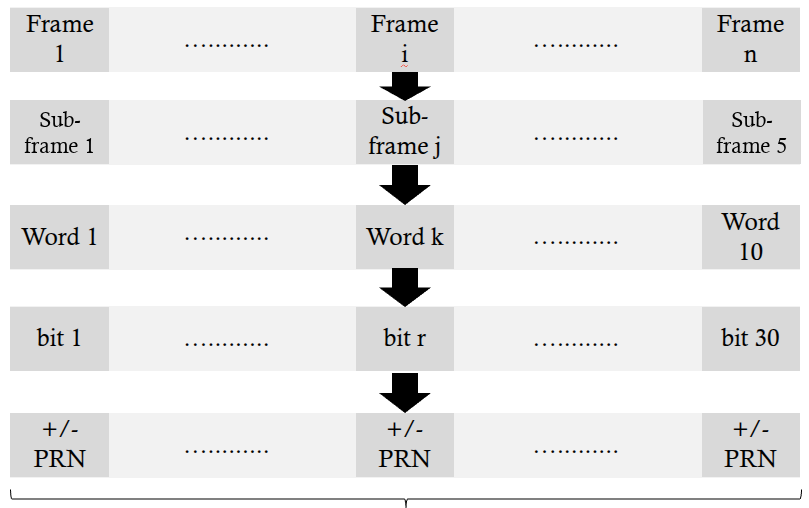
\includegraphics[width=0.8\textwidth]{GPS_struct.png}
    \caption{Structure of GPS NAV Data Hierarchy.}
    \label{fig:gps_struct}
\end{figure}

\subsection{Transmission Rate}
\begin{itemize}
  \item NAV data: 50 bits per second (bps)
  \item Each NAV bit is modulated with a PRN sequence that repeats every millisecond.
  \item Thus, each bit is spread over 20 repetitions of the PRN code (20 ms).
\end{itemize}

For better understanding of the GPS signal structure, we can refer to the IS-GPS-200K document \ref{ref:gps_struct} which provides detailed information about the GPS signal structure.

\section{PRN Codes}
\textbf{Pseudo-Random Noise (PRN)} \ref{ref:prn_generator} codes uniquely identify each GPS satellite and allow for code division multiplexing of signals.

\subsection{Key Characteristics}
\begin{itemize}
  \item Binary sequences of length 1023, repeating every 1 ms.
  \item Generated using two 10-bit Linear Feedback Shift Registers (LFSRs).
  \item The output is the modulo-2 sum of the outputs of the two LFSRs at specified tap positions (G1 and G2).
  \item The choice of G2 tap combinations determines the satellite number (SVN).
\end{itemize}

\begin{figure}[H]
    \centering
    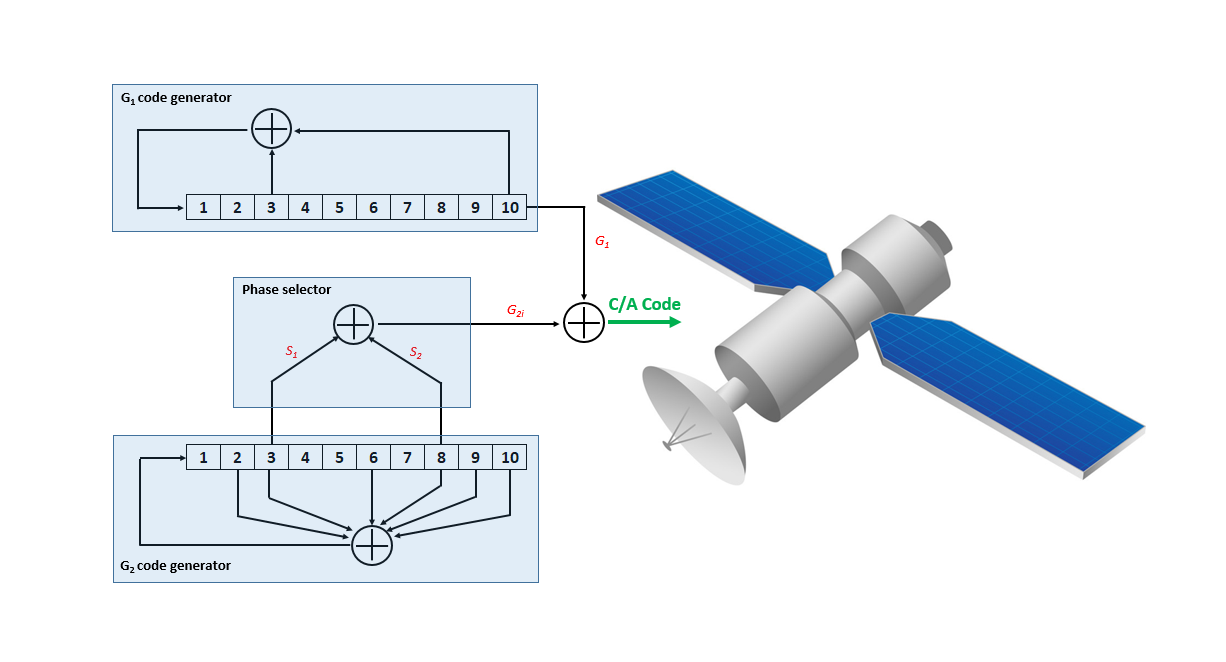
\includegraphics[width=0.8\textwidth]{PRN_gen.png}
    \caption{Generation of PRN Codes using LFSRs.}
    \label{fig:prn_gen}
\end{figure}

\subsection{Orthogonality}
\begin{itemize}
  \item PRNs are approximately orthogonal — minimal cross-correlation with others, enabling simultaneous decoding.
  \item Orthogonality allows the receiver to correlate each code separately and isolate satellite signals.
\end{itemize}

\subsection{Use in Correlation}
During acquisition and tracking, the receiver cross-correlates incoming signals with locally generated PRNs (shifted and Doppler-adjusted). Peaks in the correlation output indicate the presence and timing of specific satellites.


\section{Data Sources}
\begin{itemize}
  \item \textbf{Real-time data:} Captured using RF front ends and processed with GNSS-SDR or stored via GNU-Radio.
  \item \textbf{Real datasets:} Downloaded from public repositories.
  \item \textbf{Synthetic datasets:} Generated using GPS-SDR for controlled experimentation.
\end{itemize}

\section{GPS-SDR-SIM}
\textbf{GPS-SDR-SIM} is a software-defined GPS signal simulator that generates synthetic GPS signals for testing and research purposes. It allows users to create custom scenarios, including multiple satellites, different Doppler shifts, and various signal conditions.
\subsection{Key Features}
\begin{itemize}
  \item Generates GPS L1 C/A signals.
  \item Configurable parameters: number of satellites, Doppler shifts, signal power, and noise levels.
  \item Outputs raw I/Q samples for further processing.
  \item Useful for testing GNSS receivers and algorithms in controlled environments.
  \item Can simulate various scenarios, including multipath effects and jamming.
\end{itemize}
\subsection{Use in Experiments}
We used GPS-SDR-SIM to generate synthetic signals for our experiments, allowing us to control the parameters and conditions of the received signals. This facilitated the testing of our signal cancellation and reconstruction techniques in a controlled environment.
In our experiments, we had to control the gain of the satellite signals. To do this, in the gps-sdr-sim \ref{ref:gps_sdr_sim}, change `gpssim.c`, at line 2301, add:
\begin{verbatim}
    gain[i] = gain[i]*k;
\end{verbatim}
where `k` is the gain ratio we want to set. This allows us to control the gain of the satellite signals in the simulation. we can also change gains of each satellite individually.
\section{Experiments}

\subsection{Experiment 1: Satellite Presence Verification}
\textbf{Aim:} Verify presence of satellite 10 in the data. \\
\textbf{Method:} Upsample PRN code of satellite 10, correlate with raw data (300k samples). \\
\textbf{Result:} No visible peaks.

\begin{figure}[H]
    \centering
    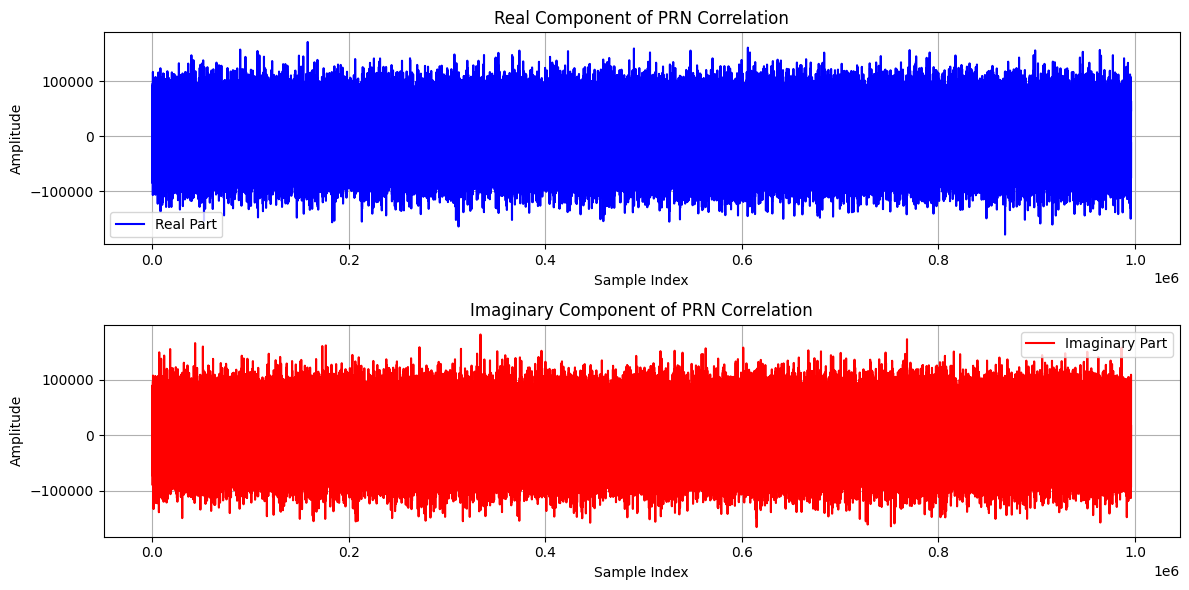
\includegraphics[width=0.6\textwidth]{exp1.png}
    \caption{Correlation results for Experiment 1.}
    \label{fig:exp1}
\end{figure}

\textbf{Analysis:} GNSS-SDR confirmed presence of satelllite 10, but we did not see the peaks. Why? Because doppler shift was not compensated in the GPS Data while correlation, thus the correlation averaged out to just the noise.


\subsection{Experiment 2: Doppler-Compensated Correlation}
\textbf{Aim:} Repeat Experiment 1 with Doppler correction. \\
\textbf{Method:} Use approx. 1 million samples. \\
\textbf{Result:} Clear peaks observed, confirming satellite presence.

\begin{figure}[H]
    \centering
    \begin{minipage}{0.48\textwidth}
        \centering
        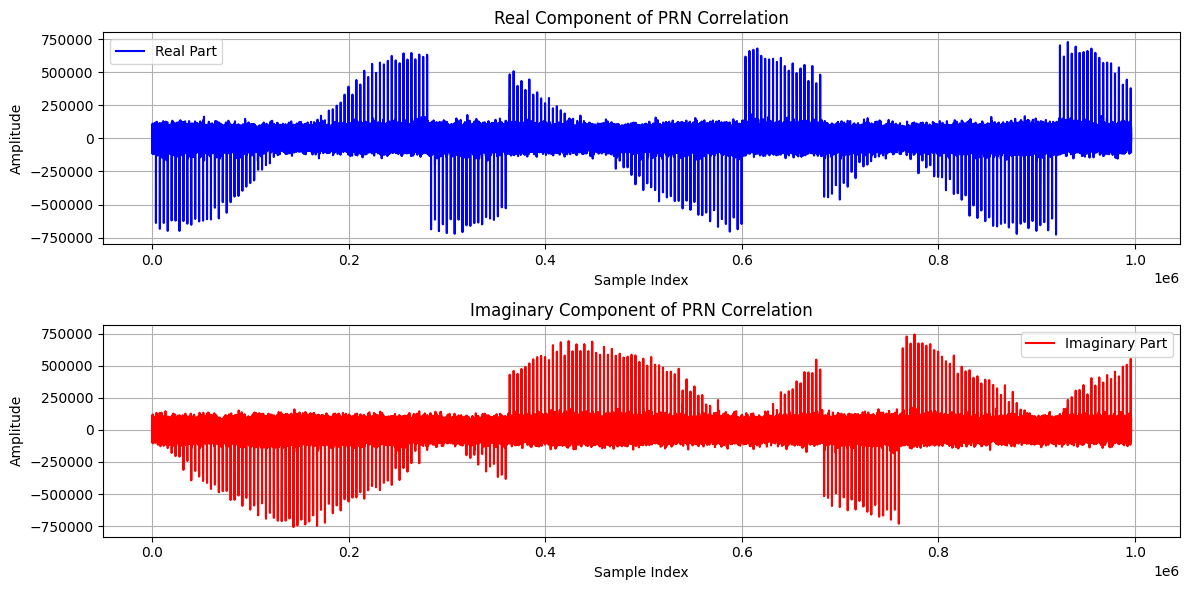
\includegraphics[width=\textwidth]{exp2.png}
        \caption{Correlation results for Experiment 2 with Doppler correction.}
        \label{fig:exp2}
    \end{minipage}
    \hfill
    \begin{minipage}{0.48\textwidth}
        \centering
        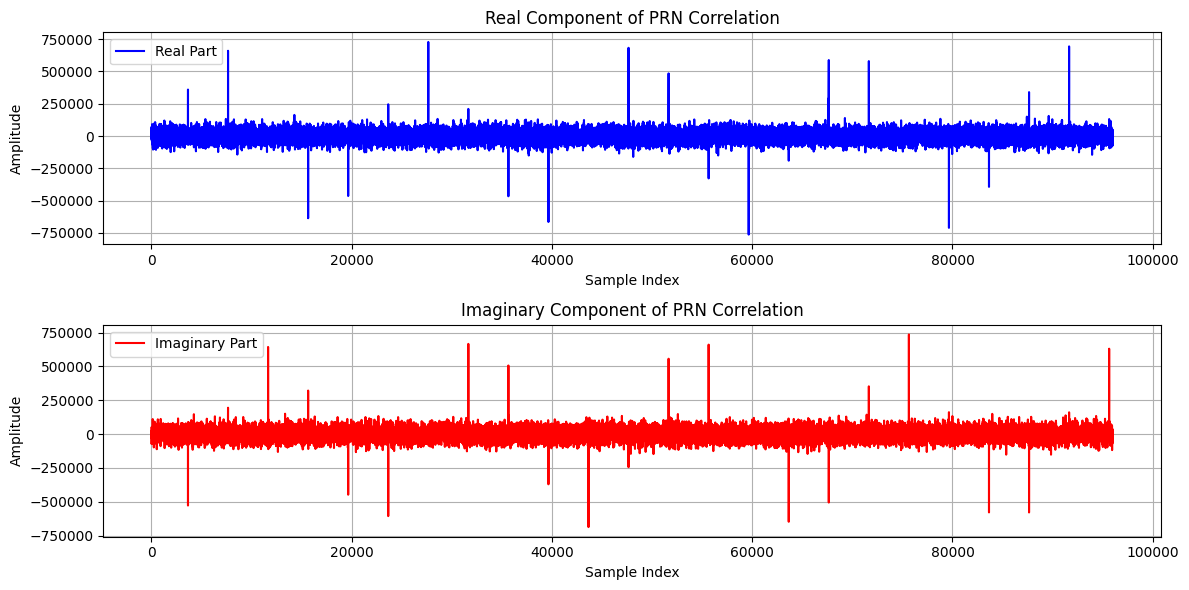
\includegraphics[width=\textwidth]{exp2_a.png}
        \caption{Doppler shift if compensated in the upsampled PRN code.}
        \label{fig:exp2_a}
    \end{minipage}
\end{figure}

\textbf{Note: }When incorporating the Doppler shift, incorporate it into the GPS Data. Do not compensate it in the upsampled PRN code 
\begin{equation}
    Y[n] = \sum_{i=1}^{N} \alpha_i x_i[n] e^{j2\pi f_{d} n/f_{s}} + \nu(n)
\end{equation}
\begin{equation}
    V[n] = PRN(10)_{upsampled}
\end{equation}
where $Y[n]$ is the received signal, $x_i[n]$ is the PRN code, $f_d$ is the Doppler frequency, and $f_s$ is the sampling frequency.
If we compensate the Doppler shift in the upsampled PRN code, we will not get the correct correlation peaks, which can be seen in these equations:
\begin{equation}
    V[n] = V[n] e^{j2\pi f_{d} n/f_{s}}
\end{equation}
\begin{equation}
    Corr = \langle Y, V\rangle 
\end{equation}
Here n in (4) will correspond to the time of the PRN code which is of the length $f_s/1000$, thus giving incorrect correlation peaks, whi
The incorrect results can be seen in the figure \ref{fig:exp2_a}. Here we dont see 20 equally spaced peaks.

\subsection{Experiment 3: Subframe Detection}
\textbf{Aim:} Detect subframe using 8-bit preamble (10001011). \\
\textbf{Challenges:} Memory issues with large datasets (4.8 GB). Takes long time to process correlation \\
\textbf{Solution:} Used \texttt{scipy.fftconvolve} to reduce processing time from hours to few minutes. Takes more memory, therefore employed chunked processing.
\begin{figure}[H]
    \centering
    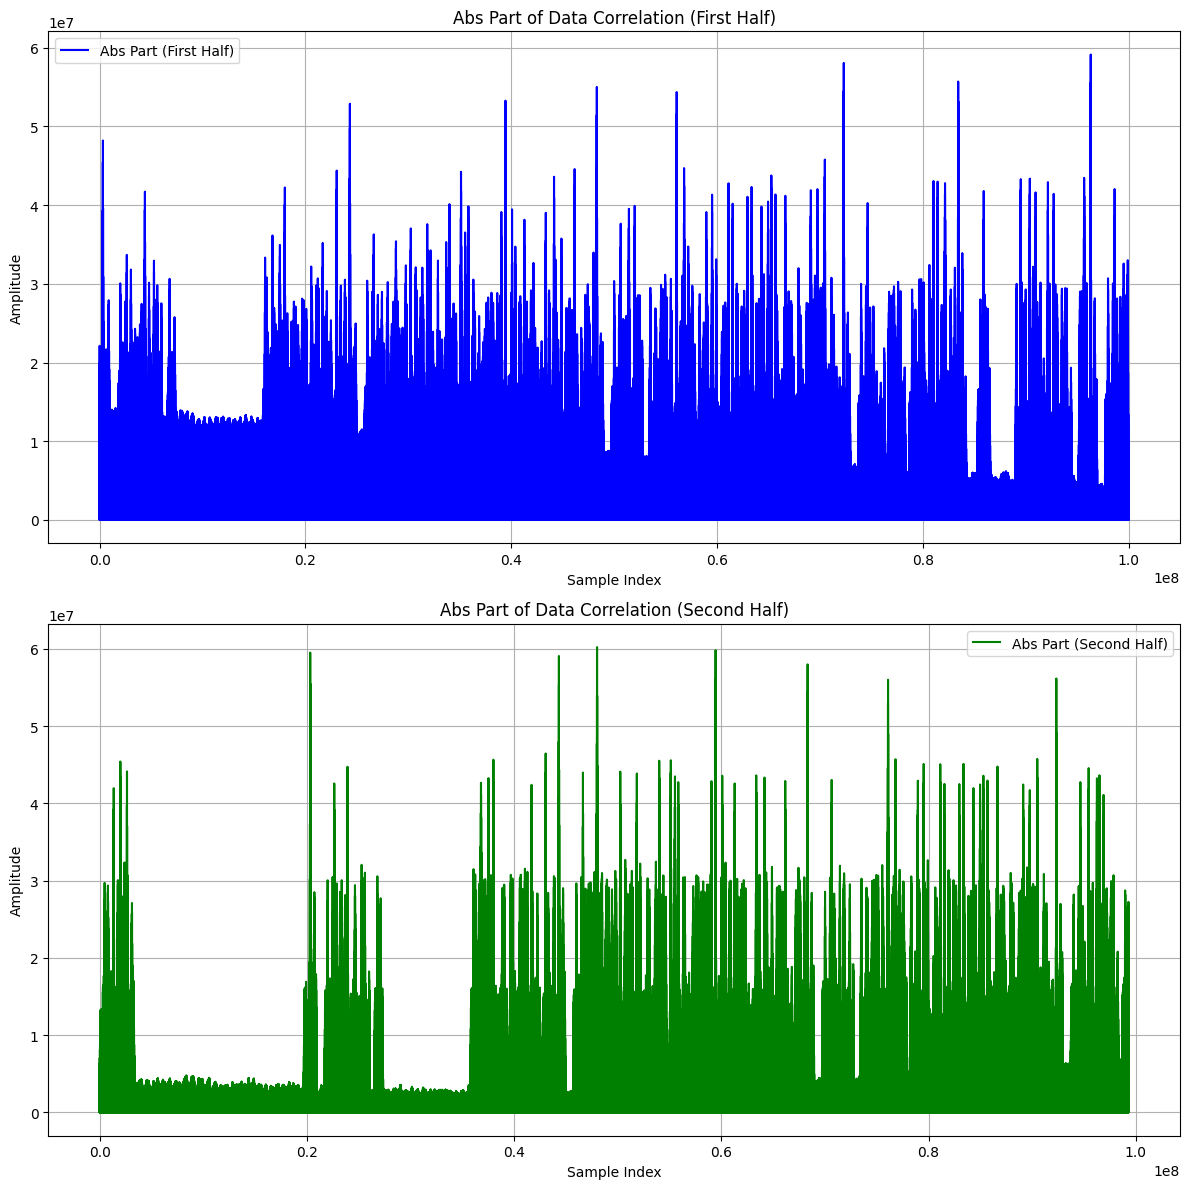
\includegraphics[width=0.6\textwidth]{exp3.png}
    \caption{Subframe detection using 8-bit preamble.}
    \label{fig:exp3}
\end{figure}

\section{Fine Doppler Correction}
Ideally doppler correction should remove imaginary peaks from the correlation, however, we still see some peaks. This is because the doppler correction is not perfect. Therefore what we did is, wrote a script which pinpoints the doppler shift to 0.01Hz accuracy. 
Now, we would expect to use the doppler shift which gives maximum absolute correlation, but because of noise, we will not get that, therefore what we do is keep a threshold for imaginary peaks (known apriori)
and then if all imaginary values are below this threshold, take the average imaginary values and then minimize it. The pseudocode is below:

\begin{algorithm}
\caption{Search Doppler Shift}
\begin{algorithmic}[1]
\REQUIRE compdata, st, chunk, fd, fs, search\_param = [$f_{min}$, step, $f_{max}$], imag\_threshold
\ENSURE best\_shift, max\_correlation

\STATE best\_shift $\leftarrow 0$
\STATE max\_correlation $\leftarrow 0$
\STATE prev\_min $\leftarrow 10^7$
\STATE curr\_min $\leftarrow 10^7$
\STATE best\_corr $\leftarrow$ None

\FOR{doppler\_shift from $f_{min}$ to $f_{max}$ with step size}
    \STATE shifted\_data $\leftarrow$ ApplyDopplerShift(compdata, fd, fs, doppler\_shift, st)
    \STATE corr $\leftarrow$ Correlate(shifted\_data, chunk)
    \STATE real\_corr $\leftarrow$ RealPart(corr)
    \STATE imag\_corr $\leftarrow$ ImagPart(corr)
    
    \IF{AllAbs(imag\_corr) $<$ imag\_threshold}
        \STATE curr\_min $\leftarrow$ Mean(Abs(imag\_corr))
        \IF{curr\_min $<$ prev\_min}
            \STATE prev\_min $\leftarrow$ curr\_min
            \STATE best\_shift $\leftarrow$ doppler\_shift
            \STATE best\_corr $\leftarrow$ DeepCopy(corr)
        \ENDIF
    \ENDIF
\ENDFOR

\IF{best\_corr is None}
    \STATE Print("No valid correlation found")
    \RETURN best\_shift, max\_correlation
\ENDIF
\RETURN best\_shift, max\_correlation

\end{algorithmic}
\end{algorithm}

The results are as follows:
\begin{figure}[H]
    \centering
    \begin{minipage}{0.48\textwidth}
        \centering
        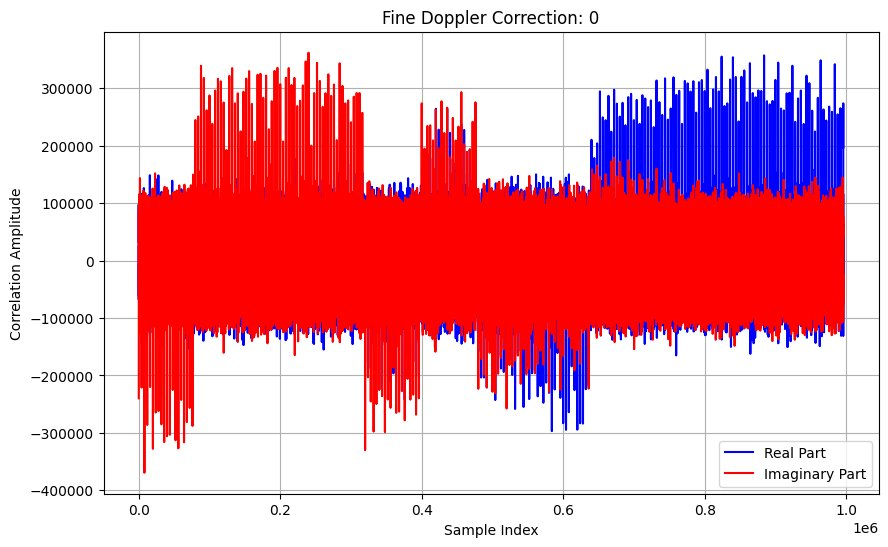
\includegraphics[width=\textwidth]{fine_dopp_a.png}
        \caption{Correlation peaks before fine Doppler correction.}
        \label{fig:fine_dop_a}
    \end{minipage}
    \hfill
    \begin{minipage}{0.48\textwidth}
        \centering
        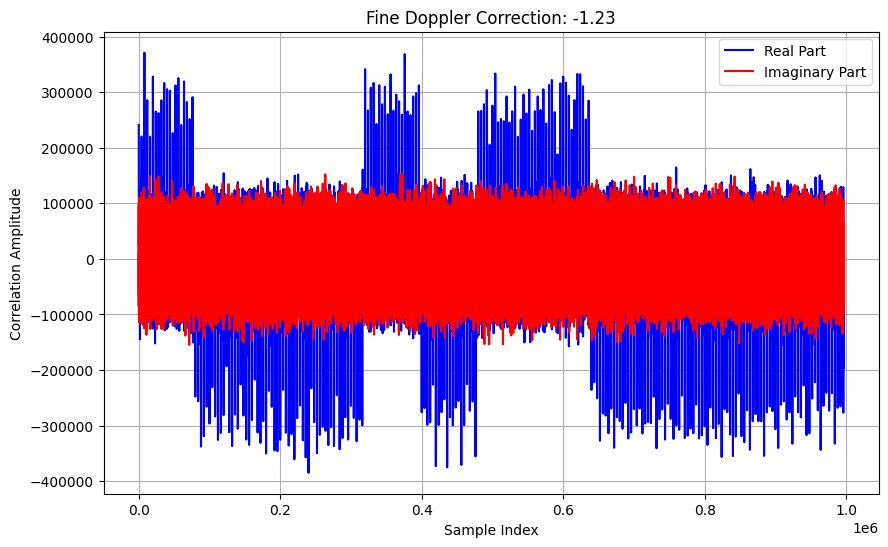
\includegraphics[width=\textwidth]{fine_dop_b.png}
        \caption{Fine Doppler correction: Real correlation peaks.}
        \label{fig:fine_dop_b}
    \end{minipage}
\end{figure}

\section{Signal Cancellation and Alpha Estimation}

\subsection{Signal Model}
Received signal: $Y = \sum \alpha_i x_i e^{j2\pi f_i t} + \text{noise}$ \\
Where:
\begin{itemize}
  \item $x_i$: known PRN sequences
  \item $f_i$: Doppler frequencies from GNSS-SDR
  \item $\alpha_i$: unknown amplitudes to be estimated
\end{itemize}

\subsection{Alpha Estimation}
We estimate $\alpha_i$ using linear regression on the correlated signal.
\begin{equation}
\boldsymbol{\alpha} = (\mathbf{X}^H \mathbf{X})^{-1} \mathbf{X}^H \mathbf{Y}
\end{equation}
Here:
\begin{itemize}
    \item $\mathbf{Y}$ is the received signal vector.
    \item $\mathbf{X}$ is the matrix of known PRN sequences modulated with Doppler shifts.
    \item $\boldsymbol{\alpha}$ is the vector of estimated amplitudes.
    \item $H$ denotes the Hermitian (conjugate transpose) operator.
\end{itemize}
For satellite 10, we estimated $\alpha$ using the correlation output. The estimated $\alpha$ values were:
\begin{itemize}
  \item \textbf{Before fine-Doppler:} $\alpha = -40.19 - 81.33j$ (unrealistic)
  \item \textbf{After fine-Doppler:} $\alpha = 94.96 + 8j$ (close to real)
\end{itemize}

\section{Verification Using GPS-SDR}
GPS-SDR was modified to set known gain values per subframe. The gain estimations were cross-verified against injected values. Visibility of satellite varied with gain ratio ($\alpha_r/\alpha_{orig}$ from 0.25 to 1.0), showing spoofing remains effective even with $\sim$70\% of true signal strength.

\section{Final Results}
Using the estimated $\alpha$, we successfully cancelled one subframe of satellite 10. GNSS-SDR was unable to decode the NAV message post-cancellation, confirming effectiveness.
\begin{figure}[H]
    \centering
    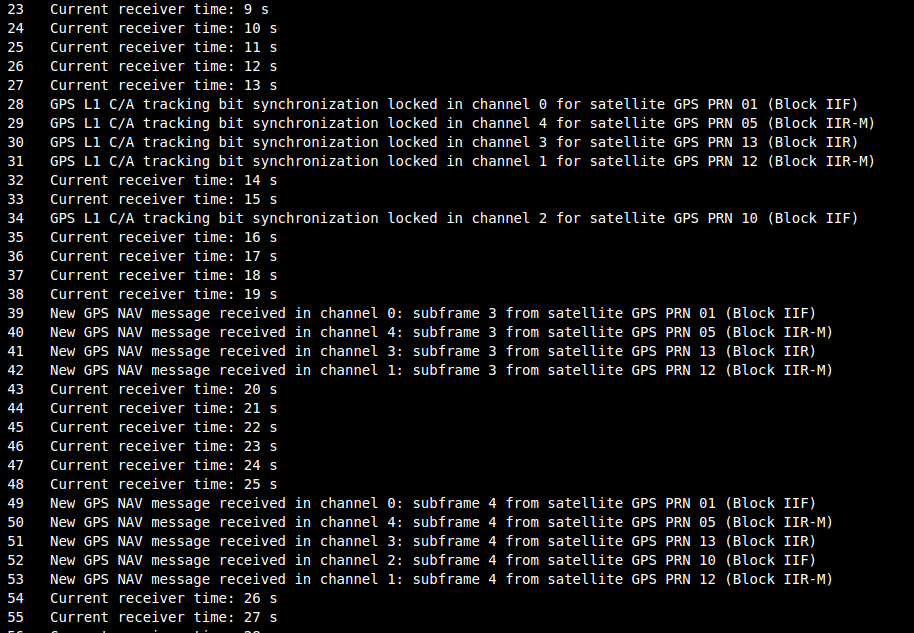
\includegraphics[width=0.6\textwidth]{cancellation.png}
    \caption{Signal cancellation results showing the absence of satellite 10's signal.}
    \label{fig:cancellation}
\end{figure}

% ... (Previous content remains unchanged until the "Future Work" section)
\noindent This was the end of BTP-1. Now as of now we are able to successfully subtract the preamble of a satellite signal. Now we shift our focus to remove the entire satellite signal from the GNSS data
given we know the decoded telemetry bits and the doppler shift data as recorded by the GNSS-SDR. We need to find an efficient way of doing this as correlating over the entire signal will take a lot of time. For this we introduce
the sliding window subtraction where we leverage the use of the fact that there is periodicity in the signal.
\section{Extended Methodology: Sliding Window Subtraction}
Given the sampling frequency $f_s$, each telemetry bit takes 20 ms to transmit, therefore each bit has $k = \frac{20f_s}{1000}$ chips. Therefore, after estimating the codephase estimate, and starting from the point where GNSS-SDR gives us the first doppler value, we start subtracting the telemetry bit.
Since each telemetry bit takes k chips, after subtacting one bit we can skip k chips ahead and start subtracting the next bit. This is done for all the telemetry bits. The code is present in the github repository, in BTP2 - main.py.

\subsection{Results}
After running the code, we ran GNSS-SDR on the output data. We tried to subtract satellite 10, but we still saw the peaks in the correlation. Why!?
\subsection{Analysis}
\begin{itemize}
  \item Improper aligning between the actual bit and its estimated position
  \item On running the codephase estimation for preambles starting position, we observed that there is a shift in the start of the subframes. Ideally, we should see that
each subframe takes 6 seconds or $6f_s$ chips which for $f_s = 4MHz$ is 24 Million samples, therefore each subframe should start after 24 million samples, but we see that each subframe starts at 24 million - 44, which is weird. 
To reproduce this run the code phase estimate function in BTP2/main.py. The data should be loaded from the gps-sdr-sim with the rinex navigation file provided in its respective repository. 
The command for reproducing the data is:

\begin{verbatim}

gps-sdr-sim -e brdc0010.22n -l 30.286502,120.032669,100 -s 4e6 -o output.dat
\end{verbatim}


  \item This means that as we move into the data there is a shift in the bits, which we were not able to figure out. Once this shift is corrected, we would be able to subtract a satellite successfully
  \item Since this is synthetic data, we believe this should not be because of the clock correction in satellites. Nevertheless, look into gps-sdr-sim code to see if they are trying to simulate the clock correction.
\end{itemize}

\begin{figure}[H]
  \centering
  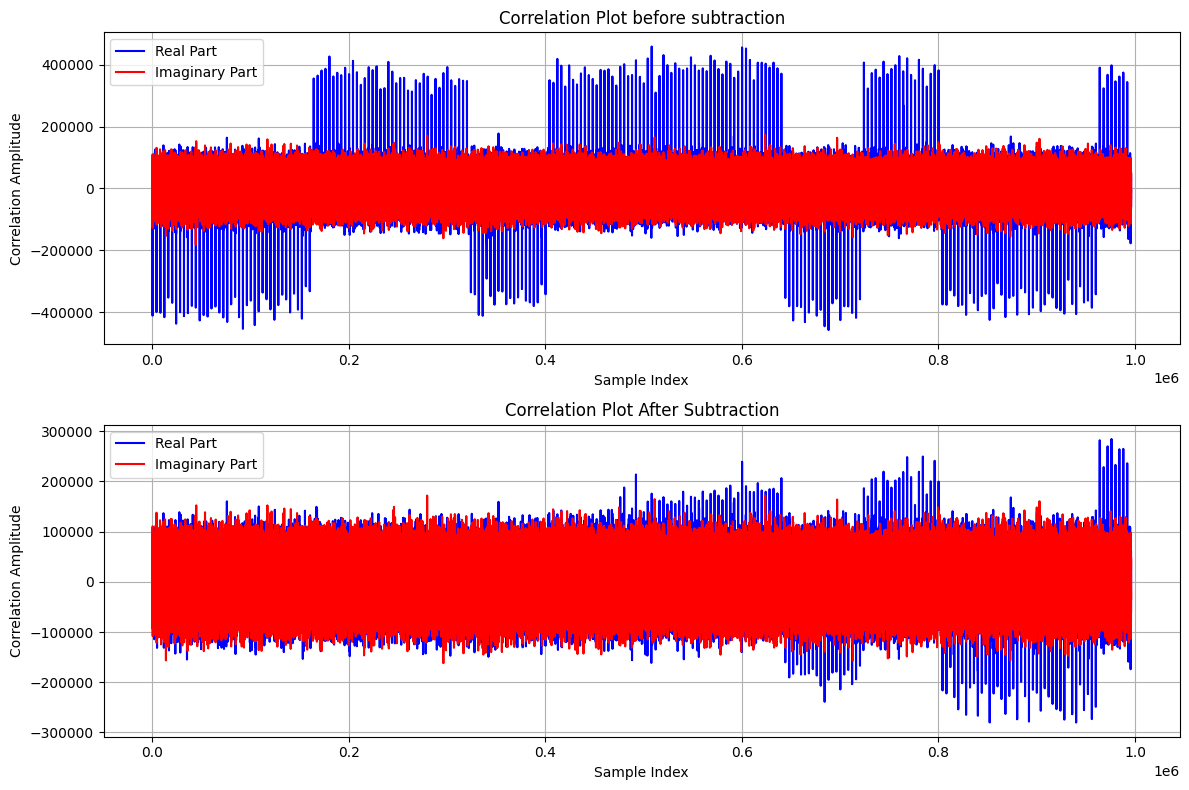
\includegraphics[width=0.6\textwidth]{misalign.png}
  \caption{So basically we started subtracting from an index lets say 100, the next PRN sequence should start at 4100, or in general 4000k + 100, if we assume $f_s = 4MHz$. If there is no shift in data, after subtraction, we should ideally see no peaks, but as we move forward with time, peaks starts resurfacing}
  \label{fig:misalign}
\end{figure}
\section{Alternate Spoofing via Signal Combination}
As cancellation proved sensitive, an alternative method was explored:
\begin{itemize}
  \item Generate two paths using \texttt{gps-sdr-sim}
  \item Create a combined signal: \( y = \alpha x_1 + (1-\alpha)x_2 \)
  \item Tune $\alpha$ until spoofed path dominates (Take minimum alpha which satisfies this condition)
  \item Generate: \( y = x_1 + \frac{1-\alpha}{\alpha}x_2 \)
\end{itemize}

\noindent How did we generate paths?
\begin{itemize}
  \item GPS-SDR-SIM's repository provides a method
  \item Go to satgen folder, there they ask us to install satgen v3
  \item Use this application to generate an NMEA facilitated
  \item Use google earth to generate a kml file which is fed into SatGen v3
  \item Finally, after producing the NMEA file, follow the steps provided in the gps-sdr-sim/satgen folder to generate a csv facilitated
  \item Then run gps-sdr-sim to generate data using the csv file
\end{itemize}

\begin{figure}[H]
  \centering
  \begin{minipage}{0.48\textwidth}
    \centering
    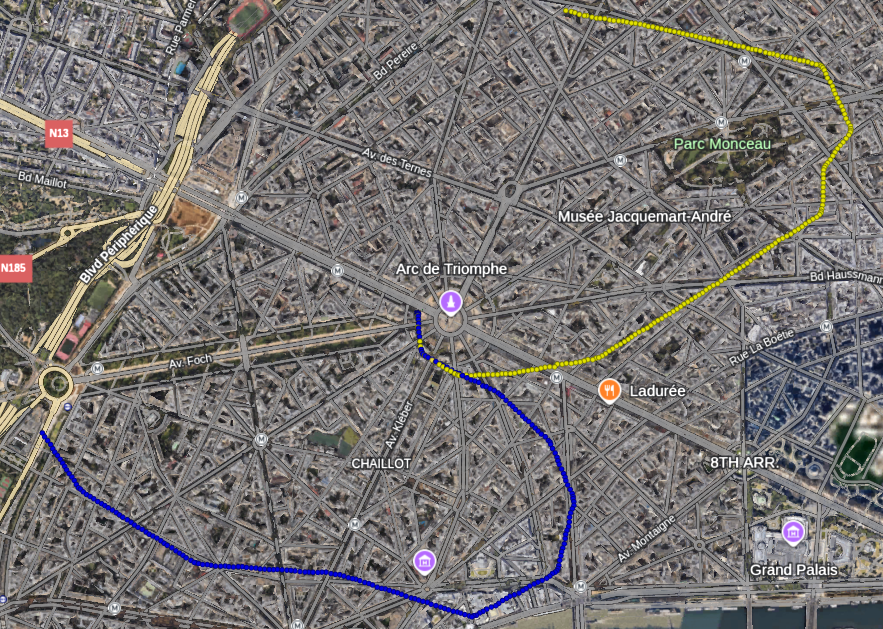
\includegraphics[width=\textwidth]{path1.png}
    \caption{Blue is the original path, yellow is the spoofed path.}
    \label{fig:path1}
  \end{minipage}
  \hfill
  \begin{minipage}{0.48\textwidth}
    \centering
    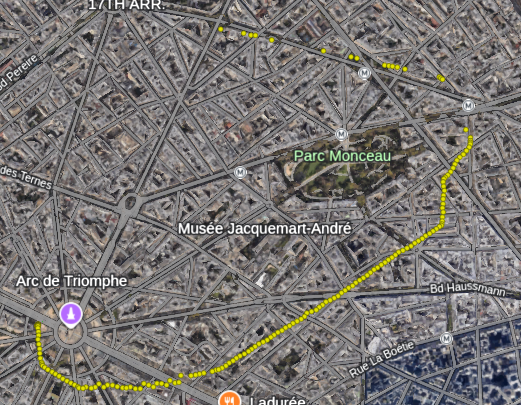
\includegraphics[width=\textwidth]{spoofed_path1.png}
    \caption{Spoofed Path}
    \label{fig:spoofed_path1}
  \end{minipage}
\end{figure}

\begin{figure}[H]
  \centering
  \begin{minipage}{0.48\textwidth}
    \centering
    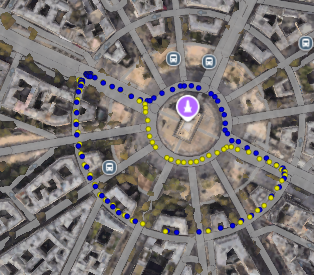
\includegraphics[width=\textwidth]{path2.png}
    \caption{Blue is spoofed path, yellow is the original path.}
    \label{fig:path2}
  \end{minipage}
  \hfill
  \begin{minipage}{0.48\textwidth}
    \centering
    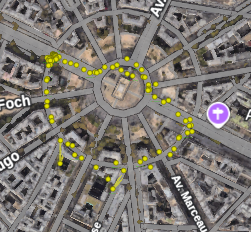
\includegraphics[width=\textwidth]{spoofed_path2.png}
    \caption{Spoofed Path}
    \label{fig:spoofed_path2}
  \end{minipage}
\end{figure}

\subsection{Results}
\begin{itemize}
  \item After running the above approach, we were able to spoof the receiver as GNSS-SDR locked on to the spoofed path
  \item Required spoofing signal to be ~50\% stronger than authentic
\end{itemize}

\noindent Since we are able to spoof a receiver, we now look into methods of anti-spoofing methods for this spoofing technique

\section{Anti-Spoofing Methodology}
Spoofing detection techniques
We can use two methods:
\begin{itemize}
  \item Compare live correlation with baseline magnitude
  \begin{itemize}
    \item if correlation is atleast twice as strong as the baseline, we can assume we are being spoofed
    \item Double because there are two signals and its reasonable to assume that spoofed signal is atleast as strong as the original signal
    \item Here baseline correlation plot is something measured in past, so it may not be reliable
  \end{itemize}
  \item Observe anomalies in PRN correlations:
      \begin{itemize}
        \item Irregular peaks
        \item Two imaginary or real peaks at the same delay
      \end{itemize}
\end{itemize}

These methods can be used to detect spoofing for the above method of spoofing.

\subsection{Observed Cases}
Dual imaginary peaks observed at:
\begin{itemize}
  \item $t = 135$ seconds
  \item $t = 180$ seconds
  \item $t = 225$ seconds
\end{itemize}

And on zooming in, at $t = 225$ we can see two different peaks shifted by a small amount. This is visble only if the real signal and spoofed signal are far apart in distance, or else the bit received would be same and hence indistinguishable.

\begin{figure}[H]
  \centering
  \begin{minipage}{0.48\textwidth}
    \centering
    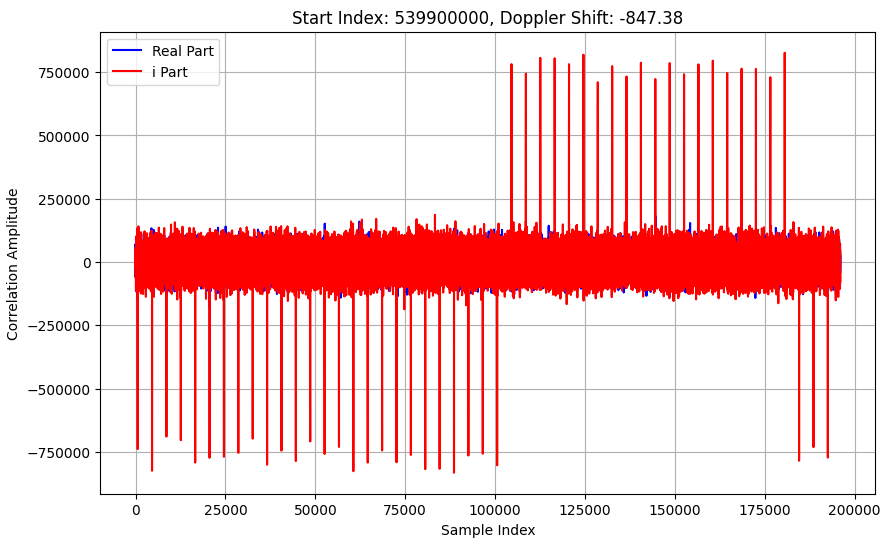
\includegraphics[width=\textwidth]{t135.png}
    \caption{Correlation peaks of original data at $t = 135$ seconds.}
    \label{fig:t135}
  \end{minipage}
  \hfill
  \begin{minipage}{0.48\textwidth}
    \centering
    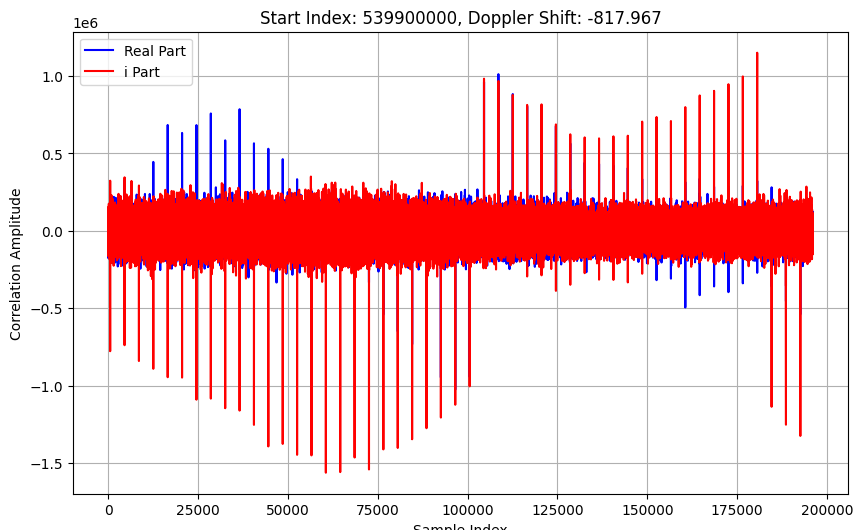
\includegraphics[width=\textwidth]{t135_sp.png}
    \caption{dual peaks at for spoofed signal $t = 135$ seconds. Not strong enough but not weak enough to be ignored.}
    \label{fig:t135_sp}
  \end{minipage}
\end{figure}

\begin{figure}[H]
  \centering
  \begin{minipage}{0.48\textwidth}
    \centering
    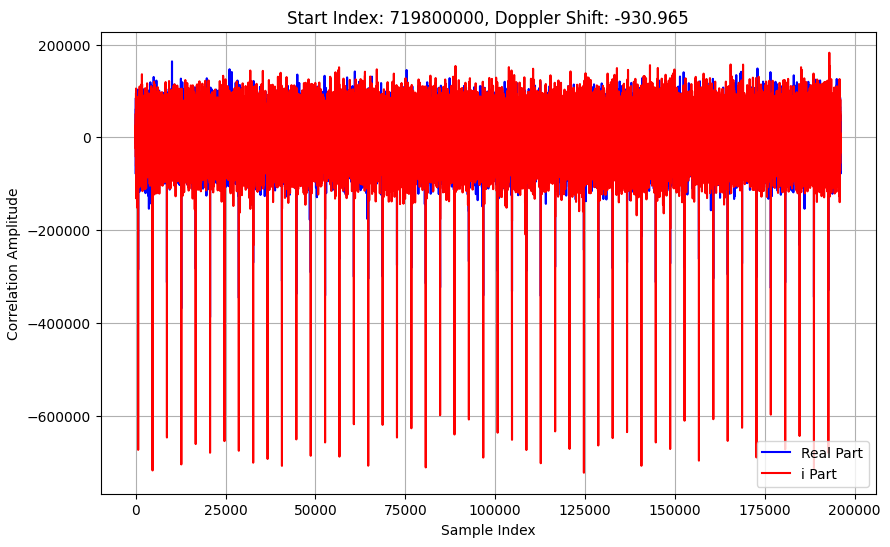
\includegraphics[width=\textwidth]{t180.png}
    \caption{Correlation peaks of original data at $t = 180$ seconds.}
    \label{fig:t180}
  \end{minipage}
  \hfill
  \begin{minipage}{0.48\textwidth}
    \centering
    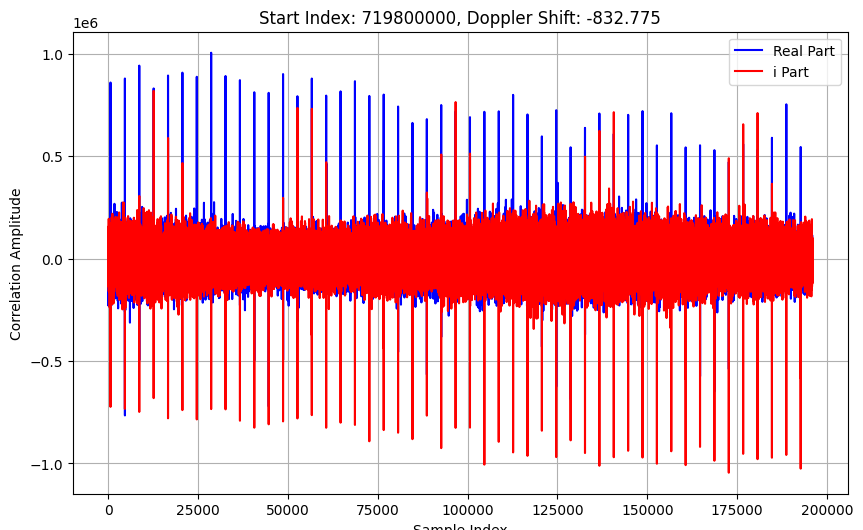
\includegraphics[width=\textwidth]{t180_sp.png}
    \caption{dual peaks at for spoofed signal $t = 180$ seconds.}
    \label{fig:t180_sp}
  \end{minipage}
\end{figure}

\begin{figure}[H]
  \centering
  \begin{minipage}{0.48\textwidth}
    \centering
    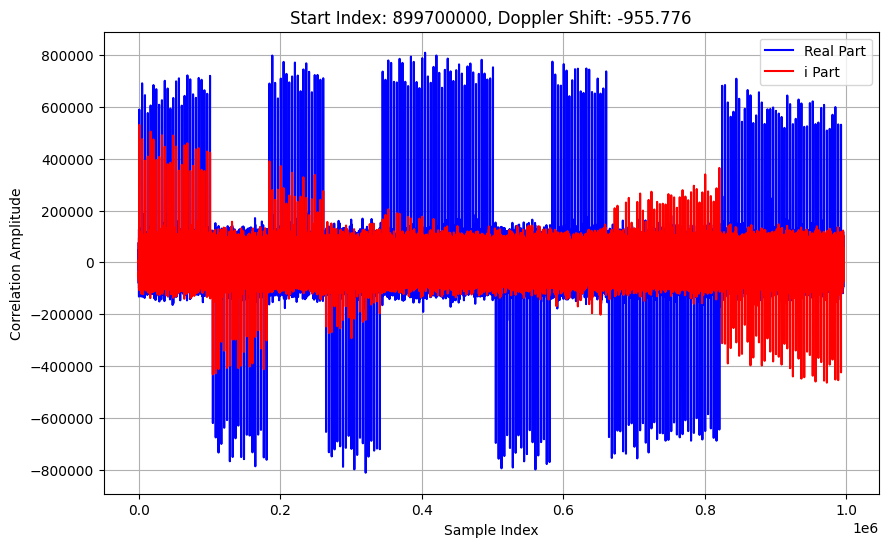
\includegraphics[width=\textwidth]{t225.png}
    \caption{Correlation peaks of original data at $t = 225$ seconds.}
    \label{fig:t225}
  \end{minipage}
  \hfill
  \begin{minipage}{0.48\textwidth}
    \centering
    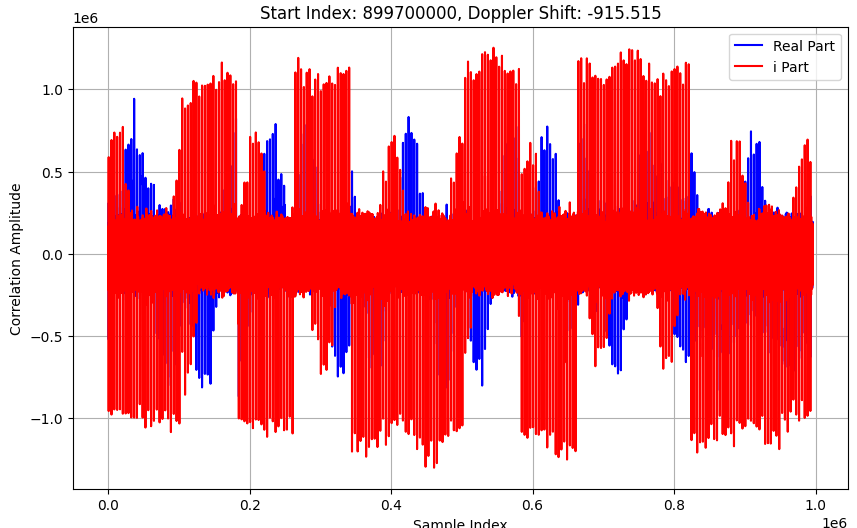
\includegraphics[width=\textwidth]{t225_sp.png}
    \caption{dual peaks at for spoofed signal $t = 225$ seconds.}
    \label{fig:t225_sp}
  \end{minipage}
\end{figure}

\begin{figure}[H]
  \centering
  \begin{minipage}{0.32\textwidth}
    \centering
    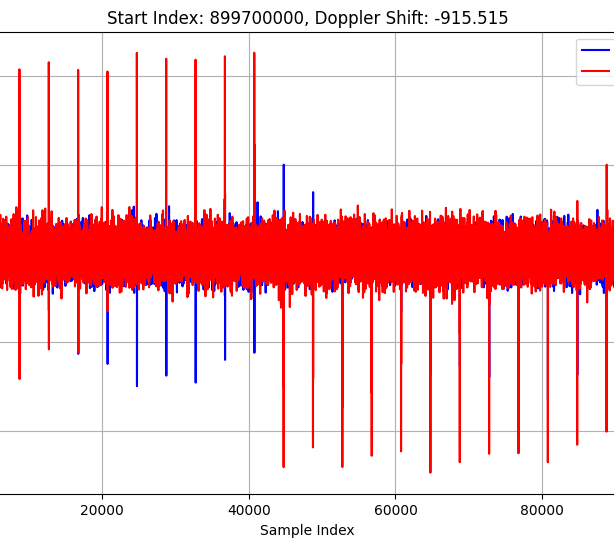
\includegraphics[width=\textwidth]{t225_z1.png}
    \caption{Zoomed-in view of correlation peaks at $t = 225$ seconds (Region 1).}
    \label{fig:t225_z1}
  \end{minipage}
  \hfill
  \begin{minipage}{0.32\textwidth}
    \centering
    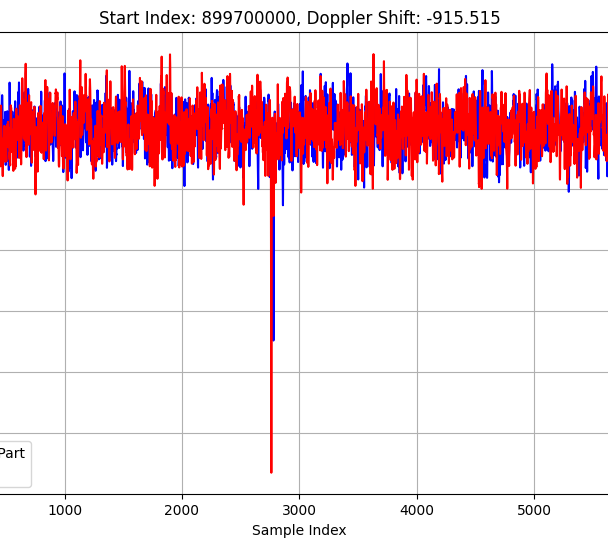
\includegraphics[width=\textwidth]{t225_z2.png}
    \caption{Zoomed-in view of correlation peaks at $t = 225$ seconds (Region 2).}
    \label{fig:t225_z2}
  \end{minipage}
  \hfill
  \begin{minipage}{0.32\textwidth}
    \centering
    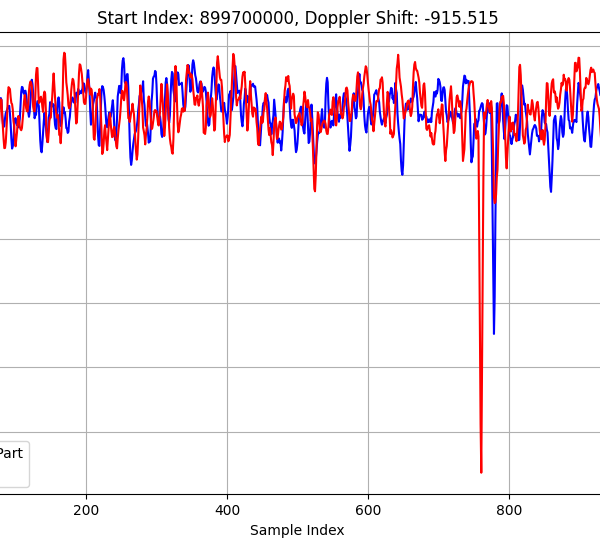
\includegraphics[width=\textwidth]{t225_z3.png}
    \caption{Zoomed-in view of correlation peaks at $t = 225$ seconds (Region 3).}
    \label{fig:t225_z3}
  \end{minipage}
\end{figure}

These confirm presence of superimposed signals.

\section{Miscellaneous Experiments}
We plotted estimated $\alpha$ from a GNSS signal simulated by gps-sdr-sim, vs the actual gain values with which we simulated the signal.:
\begin{itemize}
  \item Observed near-linear relationship
  \item Helps plan spoofing gain given fine Doppler info
\end{itemize}

\begin{figure}[H]
  \centering
  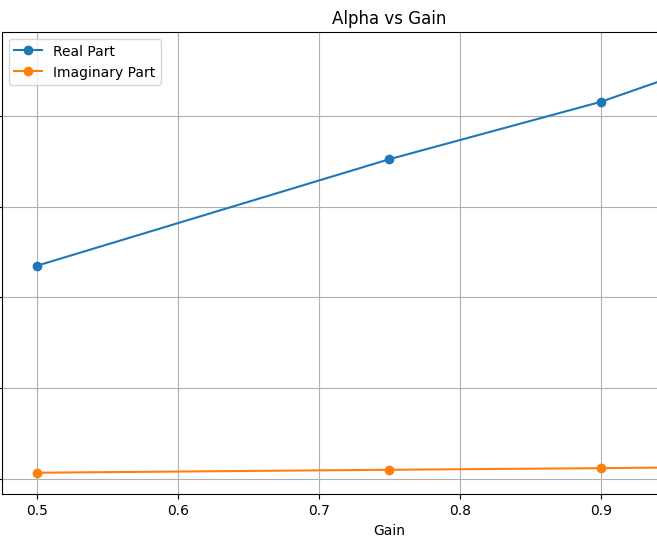
\includegraphics[width=0.6\textwidth]{alpvsgain.png}
  \caption{Estimated $\alpha$ vs Actual Gain Values.}
  \label{fig:alpvsgain}
\end{figure}

\section{Conclusions}
\begin{itemize}
  \item Satellite signals can be cancelled or overlaid for spoofing
  \item Fine Doppler correction is critical for alignment
  \item Linear combination enables spoofing with stronger secondary signals
  \item Anomalies in correlation allow spoof detection
\end{itemize}

\section{Future Work}
\begin{itemize}
  \item Real-time spoofing and anti-spoofing pipelines
  \item Analyze long-term variations in correlation peaks
  \item Efficient signal subtraction over multiple frames
\end{itemize}

\section{References}
\begin{enumerate}
    \item \label{ref:gnss_sdr} GNSS-SDR: An open-source GNSS software-defined receiver. Retrieved from \url{https://gnss-sdr.org/}
    \item \label{ref:gps_struct} GPS Signal Structure: Understanding the GPS signal structure. Retrieved from \url{https://www.gps.gov/technical/icwg/IS-GPS-200K.pdf}
    \item \label{ref:prn_generator} PRN Generator: A tool for generating PRN codes. Retrieved from \url{https://natronics.github.io/blag/2014/gps-prn/}
    \item \label{ref:gps_sdr_sim} GPS-SDR-SIM: An open-source GPS signal simulator. Retrieved from \url{https://github.com/osqzss/gps-sdr-sim}
\end{enumerate}

\section{Acknowledgements}
We would like to thank Prof. Sibiraj Pillai for his guidance throughout this project.

\end{document}

